\documentclass[12pt,utf8,notheorems,compress,t,aspectratio=169]{beamer}
\usepackage{etex}
\usepackage{pgfpages}
\usepackage{calc}
\usepackage[export]{adjustbox}
\usepackage[english]{babel}
\usepackage[normalem]{ulem}
\usepackage{mathtools}
\usepackage{booktabs}
\usepackage{stmaryrd}
\usepackage{amssymb}
\usepackage{manfnt}
\usepackage{array}
\usepackage{ragged2e}
\usepackage{multicol}
\usepackage{tabto}
\usepackage{xstring}
\usepackage{xspace}
\usepackage{proof}
\usepackage[all]{xy}
\xyoption{rotate}
\usepackage{tikz}
\usetikzlibrary{tikzmark,decorations.pathreplacing,calc,shapes,shapes.callouts,shapes.arrows,patterns,fit,backgrounds,decorations.pathmorphing,positioning,svg.path}
\hypersetup{colorlinks=true}
\usepackage[protrusion=true,expansion=true]{microtype}
\usepackage{pifont}
\usepackage[skins]{tcolorbox}

\setbeamersize{text margin left=1.60em,text margin right=1.60em}

% Workaround for the issue described at
% https://tex.stackexchange.com/questions/164406/beamer-using-href-in-notes
\newlength\tbheight
\newcommand{\fixedhref}[2]{%
  \begingroup%
    \setlength{\tbheight}{\heightof{\phantom{#2}}}
    \parbox[t][0pt][t]{0pt}{%
      \hfuzz=\maxdimen%
      \vspace*{-\paperheight}%
      \vspace*{-\tbheight}%
      \vbox{\href{#1}{\phantom{#2}}}%
    }%
    #2%
  \endgroup%
}

% from Dominik Kirst
\newtcolorbox{emptybox}{
  beamer,
  width=(0.62\textwidth),
  % enlarge left by=-3pt,
  titlerule=0mm,
  colframe=white,
  coltitle=black,
  bottom=6pt,
  top=-12pt,
  left=6pt,
  right=6pt,
  notitle,
  adjusted title={},
  outer arc=.5mm,
  arc=.5mm,
  no shadow,
  fuzzy shadow={1mm}{-1mm}{-1.2mm}{.7mm}{black!20},
  interior titled code={}
}

\newcommand{\cmark}{\ding{51}}
\newcommand{\xmark}{\ding{55}}
\DeclareSymbolFont{extraup}{U}{zavm}{m}{n}
\DeclareMathSymbol{\varheart}{\mathalpha}{extraup}{86}

\graphicspath{{images/}}

\setlength\parskip{\medskipamount}
\setlength\parindent{0pt}

\title{Three bizarre logico-philosophical tales about the axiom of choice}

\author{Ingo Blechschmidt}
\date{December 27th, 2023}

\setbeameroption{show notes on second screen=bottom}
\newcommand{\jnote}[2]{\only<#1>{\note{\usebackgroundtemplate{x}\setlength\parskip{\medskipamount}\footnotesize\justifying#2\par}}}
\setbeamertemplate{note page}[plain]

\useinnertheme{rectangles}

\usecolortheme{seahorse}
\definecolor{mypurple}{RGB}{253,73,34}
\definecolor{mypurpledark}{RGB}{100,0,150}
\setbeamercolor{structure}{fg=mypurple}
\setbeamercolor*{title}{bg=mypurple,fg=white}
\setbeamercolor*{titlelike}{bg=mypurple,fg=white}
\setbeamercolor{frame}{bg=black}
\setbeamertemplate{blocks}[rounded][shadow=true]

\usefonttheme{serif}
\usepackage[T1]{fontenc}
\usepackage{libertine}

\newcommand{\NN}{\mathbb{N}}
\newcommand{\RR}{\mathbb{R}}

\setbeamertemplate{frametitle}{%
  \leavevmode%
  \vskip-1.6em%
  \begin{beamercolorbox}[dp=1ex,center,wd=\paperwidth,ht=2.25ex]{title}%
    \vskip0.5em%
    \bf\insertframetitle
  \end{beamercolorbox}%

  \vskip-0.77em\hspace*{-2em}%
  \textcolor{mypurpledark}{\rule[0em]{1.1\paperwidth}{2.4pt}}

  \vskip-0.4em%
}

\setbeamertemplate{navigation symbols}{}

\newcommand{\insertframeextra}{}
\setbeamertemplate{footline}{%
  \begin{beamercolorbox}[wd=\paperwidth,ht=2.25ex,dp=1ex,right,rightskip=1mm,leftskip=1mm]{}%
    % \inserttitle
    \hfill
    \insertframenumber\insertframeextra\,/\,\inserttotalframenumber
  \end{beamercolorbox}%
  \vskip0pt%
}

\newcommand{\hil}[1]{{\usebeamercolor[fg]{item}{\textbf{#1}}}}
\newcommand{\bad}[1]{\textcolor{red!90}{\textnormal{#1}}}
\newcommand{\good}[1]{\textcolor{mypurple}{\textnormal{#1}}}

\newcommand{\normalnumber}[1]{%
  {\renewcommand{\insertenumlabel}{#1}\!\usebeamertemplate{enumerate item}\!}
}
\newcommand{\bignumber}[1]{%
  \renewcommand{\insertenumlabel}{#1}\scalebox{1.2}{\!\usebeamertemplate{enumerate item}\!}
}

\begin{document}

\addtocounter{framenumber}{-1}

{\usebackgroundtemplate{\begin{minipage}{\paperwidth}\centering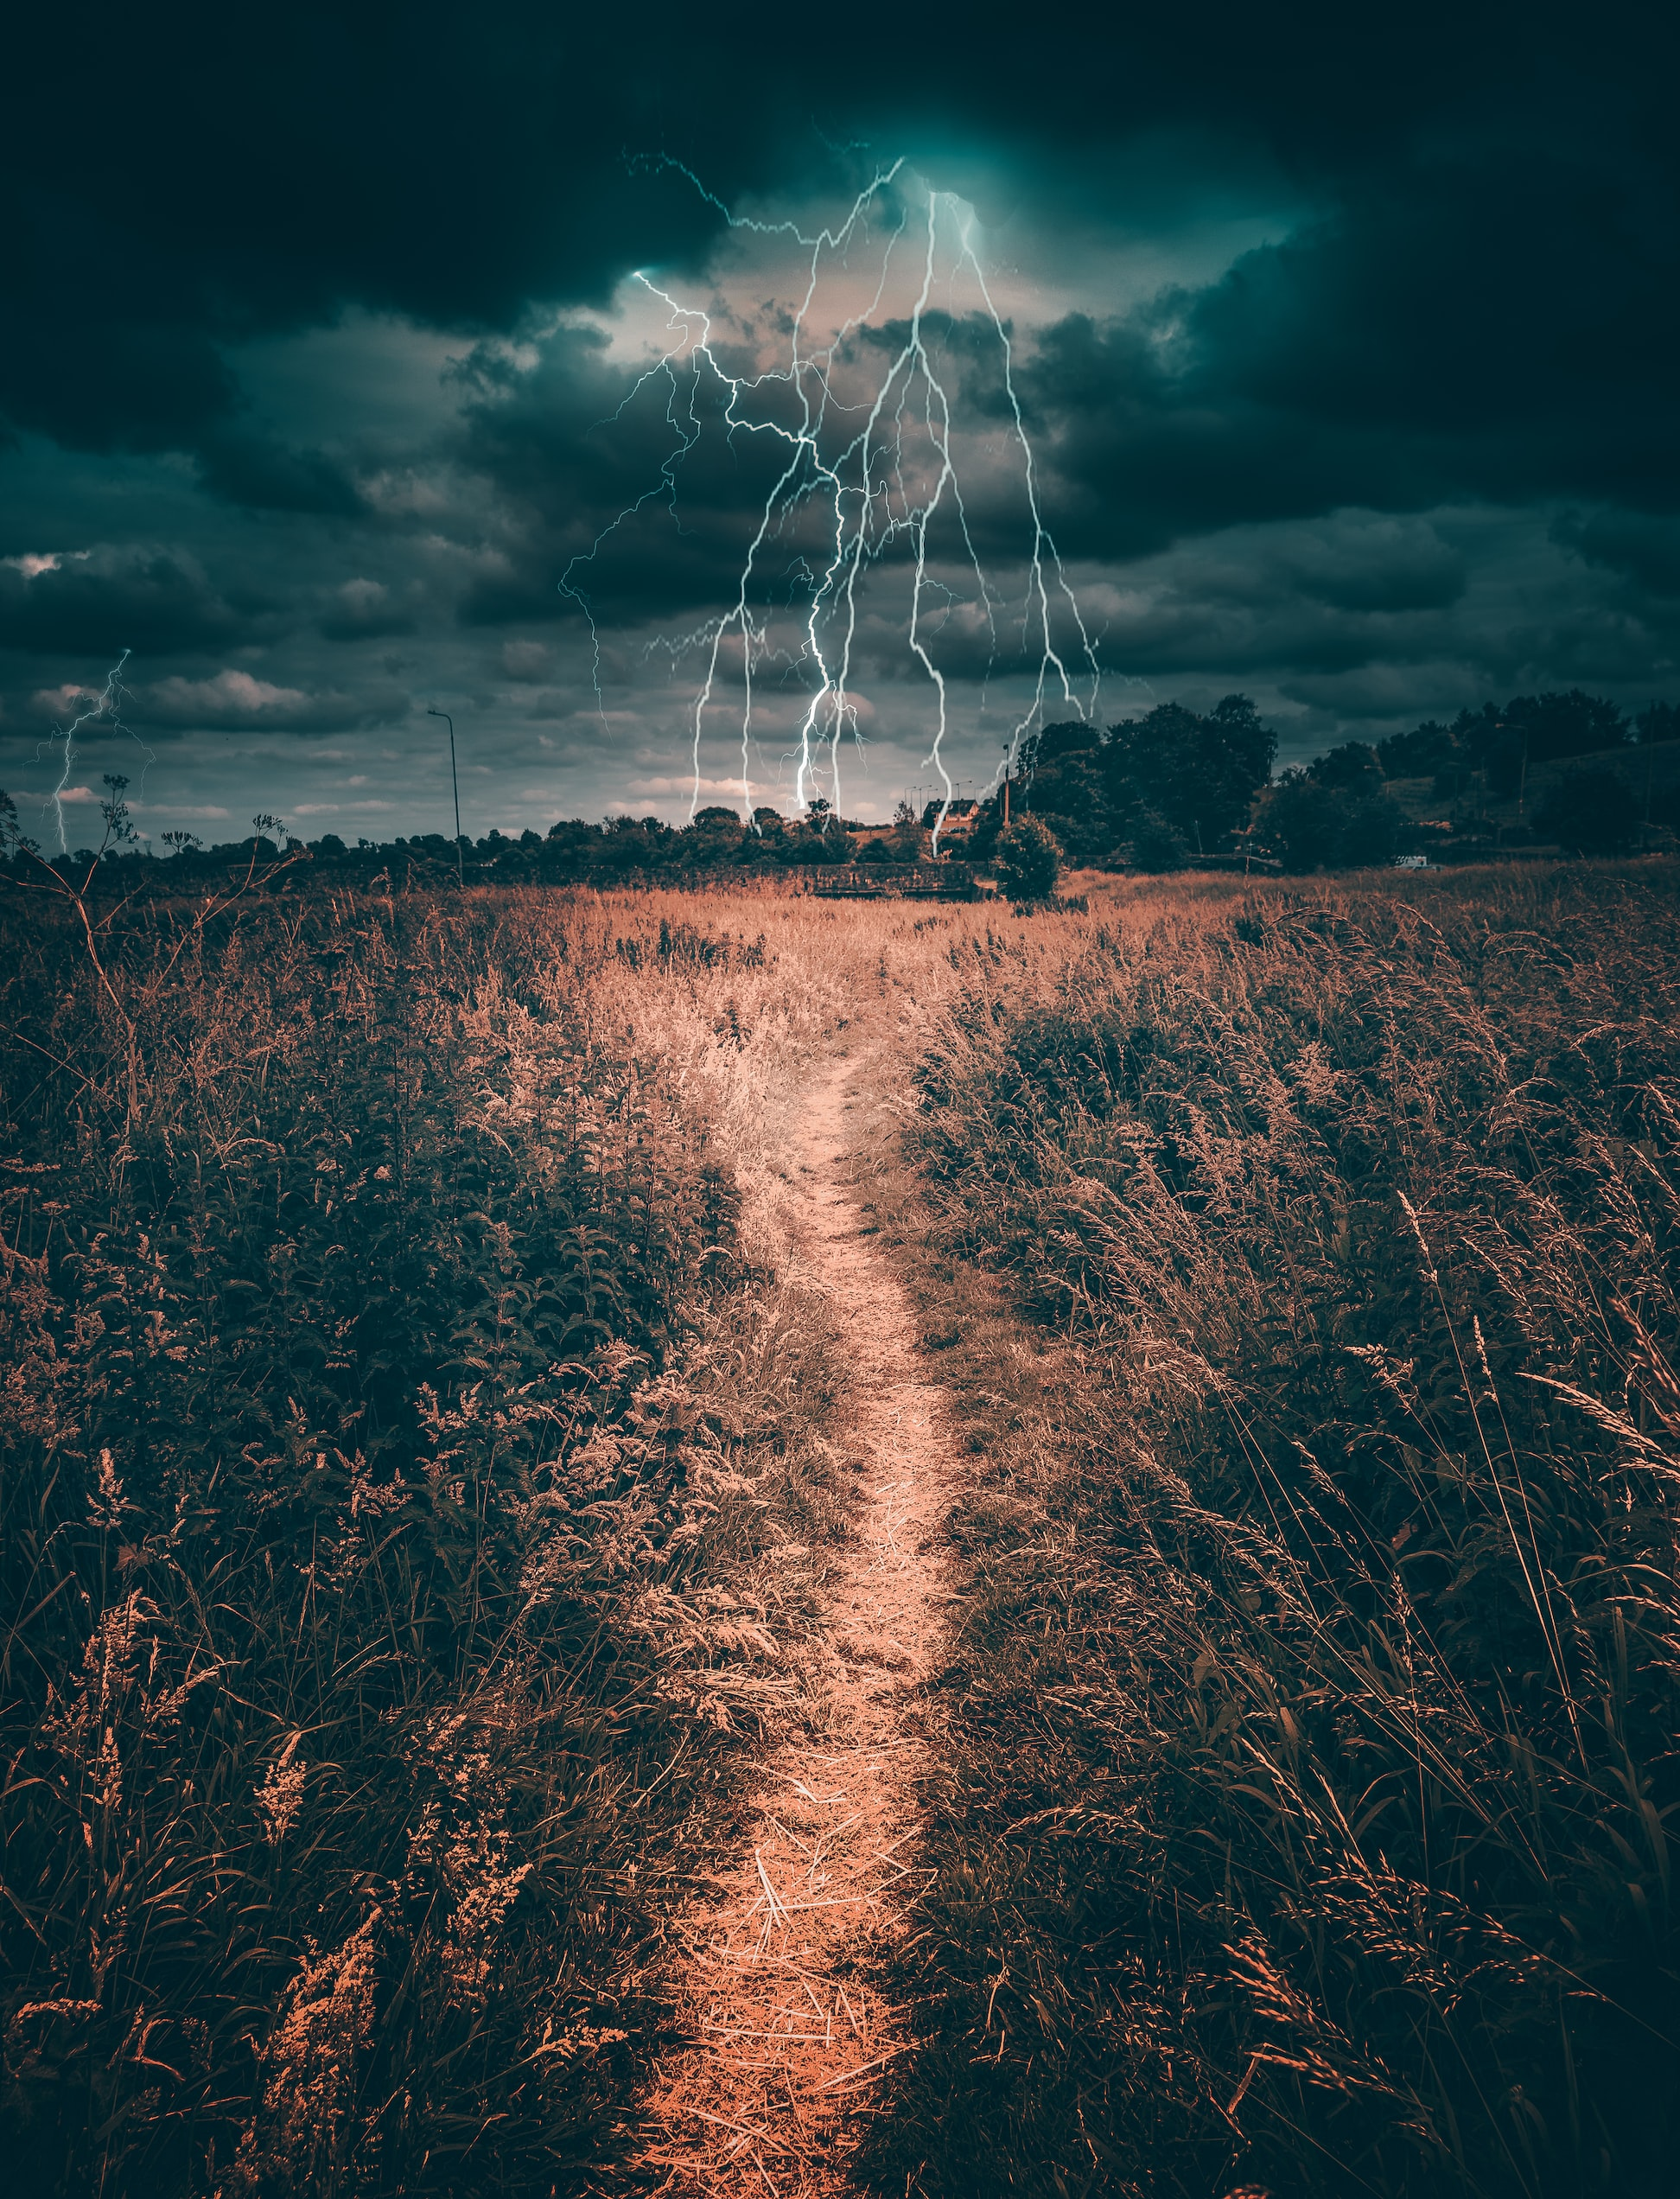
\includegraphics[width=\paperwidth]{lightning}\end{minipage}}
\begin{frame}[c]
  \jnote{2-}{
    An evil monster conjures numbers atop all members of an infinite team of
    mathematicians. They can see and cognitively process the numbers placed on
    everyone else, but are strictly forbidden to peek at their own number.
    Instead, the monster will ask every one of them to privately venture a
    guess regarding the value of their number.

    Is there a strategy which, if followed by the mathematicians, ensures that
    \emph{only finitely many} of them guess their number incorrectly? The
    strategy must be universal, applicable regardless of the specific numbers
    assigned by the monster.

    Communication among the team is allowed only beforehand. Nothing is known
    about the distribution of numbers chosen by the monster. Also note that
    infinitely many mathematicians being right does not yet mean that only finitely many
    guess incorrectly. For instance, if every second guess is right, then every
    other second guess is incorrect.
  }

  \jnote{3-}{
    The challenge posed by the monster seems impossible to satisfy: The monster
    is free in its distribution of numbers; observing the numbers hovering on
    all the other mathematicians does not restrict the amount of possibilities
    for your own number in any way.

    Surprisingly, despite appearances, there does exist a suitable winning strategy---%
    if and only if (a certain instance of) the axiom of choice holds.
  }

  \centering

  \bigskip
  \bigskip
  \bigskip
  \bigskip

  \scriptsize

  \setbeamercolor{block body}{bg=black!100}
  \begin{minipage}{0.62\textwidth}
    \begin{block}{}
      \centering\normalsize\color{white}
      \hil{\phantom{g}Three bizarre logico-philosophical tales \\ about the axiom of
      choice\phantom{g}}
    \end{block}
  \end{minipage}

  \color{white}
  \textit{-- an invitation --}

  \vspace*{9.9em}
  \raisebox{0pt}[0pt][0pt]{\hspace*{-2.4em}\begin{minipage}[0em]{\paperwidth}\centering%
    \only<1>{
      Ingo Blechschmidt \medskip

      37th Chaos Communication Congress \\
      December 27th, 2023
    }
    \only<2->{\fixedhref{https://www.spikedmath.com/}{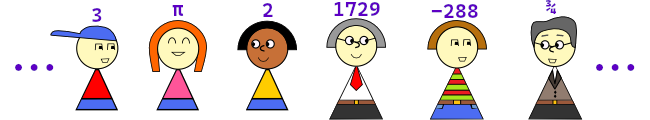
\includegraphics[width=\paperwidth]{long-queue}}}
  \end{minipage}}
\end{frame}}

\definecolor{mypurple}{RGB}{150,0,255}
\setbeamercolor{structure}{fg=mypurple}

{\usebackgroundtemplate{\begin{minipage}{\paperwidth}\centering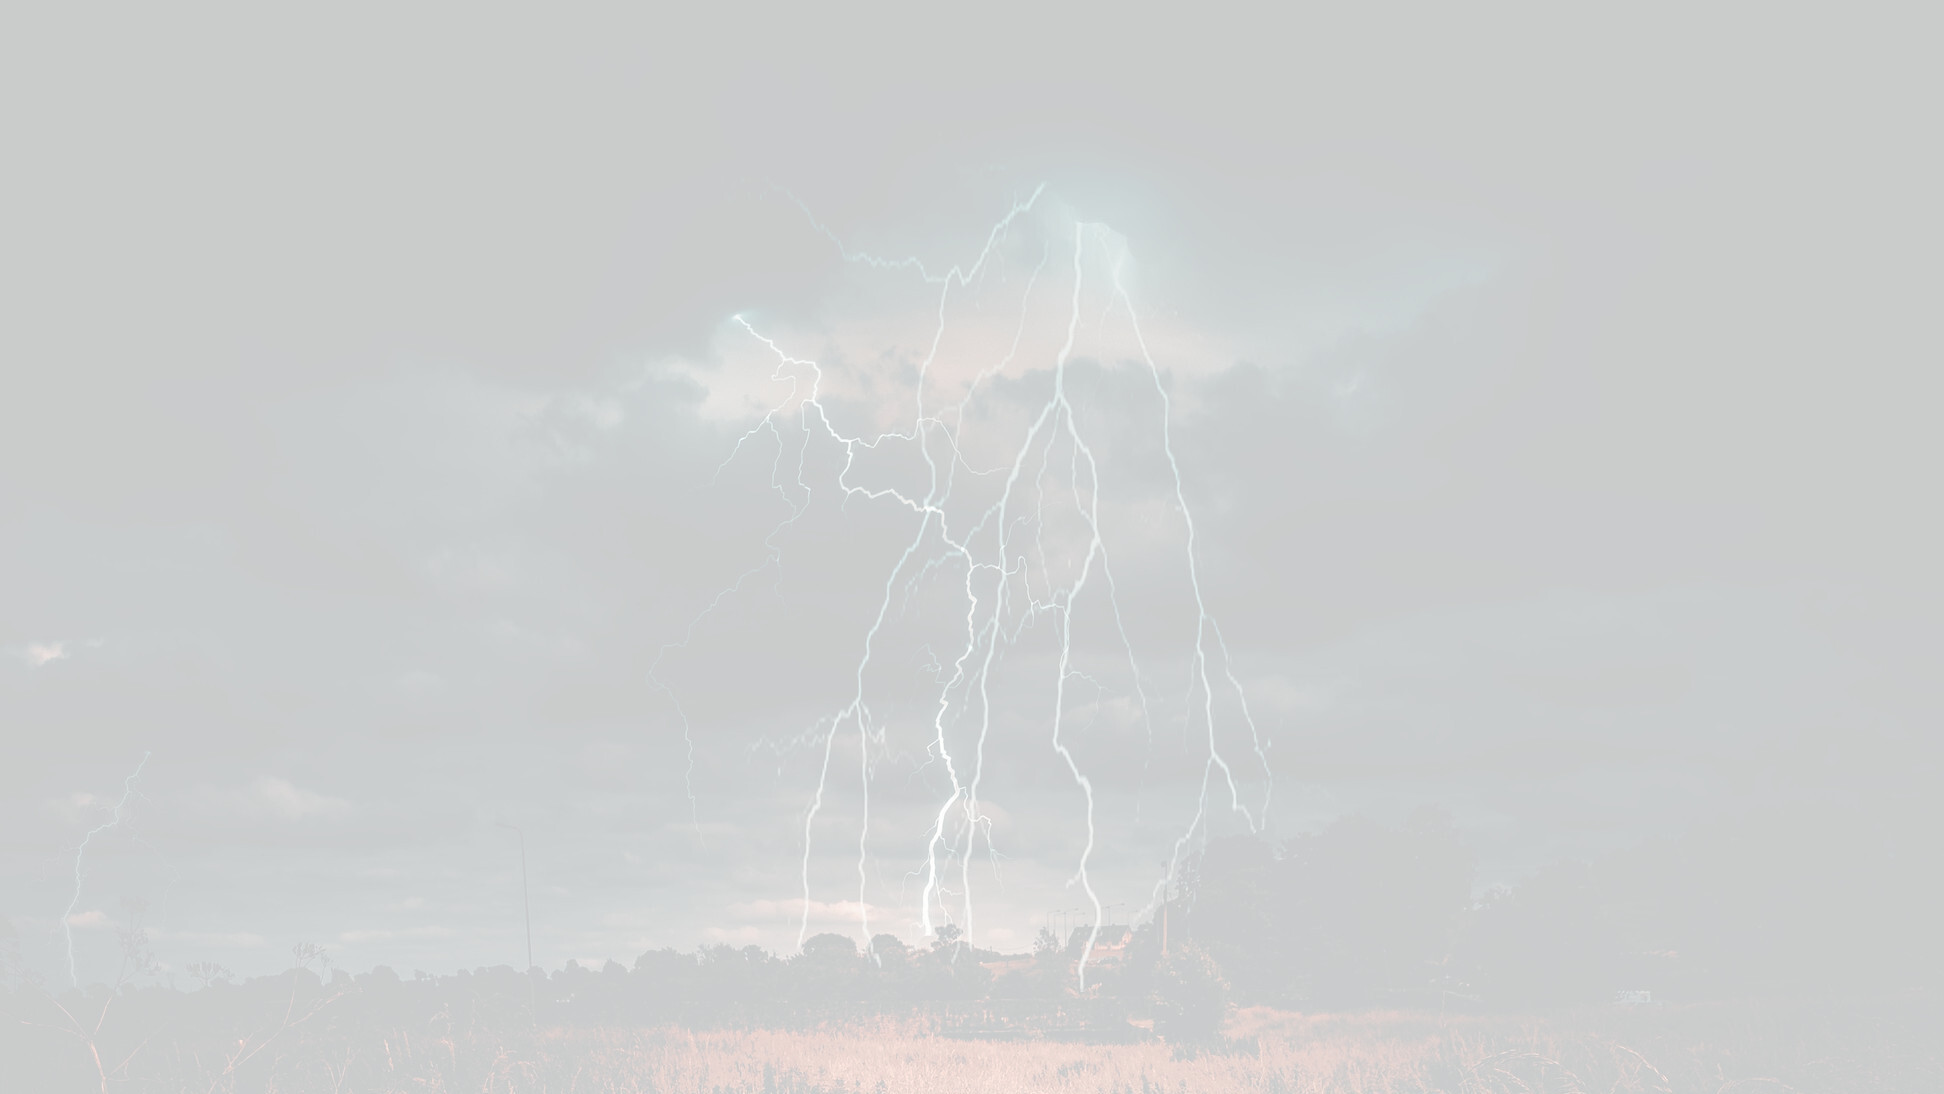
\includegraphics[width=\paperwidth]{lightning-lighter}\end{minipage}}
\begin{frame}{Choice functions}
  \jnote{1-}{
    The slide uses the terms ``collection'' and ``set'' interchangeably. A set
    is called ``inhabited'' if and only if it contains at least one element.
  }

  \jnote{2-}{
    By ``function'', we always mean pure deterministic function. Hence
    JavaScript's \textsf{document.getElementById} is only an example if
    the DOM never changes.
  }

  \jnote{3-}{
    The two examples for choice functions provided on the slide don't compute
    arbitrary representatives, but representatives which are singled out by
    special properties---being the mayor or being the youngest member. However,
    choice functions are also allowed to return representatives with no
    discernible special attributes.
  }

  \jnote{4-}{
    In case~A, we could just write down a full specification of a choice
    function by randomly drawing representatives. In order for the resulting
    choice function to be deterministic, as required for functions, the random
    sampling needs to be done once, beforehand, not anew for each call.

    In case~B, the function which computes the smallest
    possible representatives is a suitable choice function.
  }

  \setbeamercolor{block body}{bg=white!100}
  {\centering\emph{\scriptsize The axiom of choice (\textsc{ac}) asserts:}\\[-0.5em]\begin{emptybox}
    \centering
    ``For \hil{every} collection of inhabited sets, \\
    there is a \hil{choice function} picking \\
    \hil{representatives} from each set.''
  \end{emptybox}\par}
  \bigskip
  \pause

  Examples for functions:
  \vspace*{-0.2em}
  \begin{enumerate}
    \small
    \item sine function: $x \mapsto \sin(x)$
    \item squaring function: $x \mapsto x^2$, so $1 \mapsto 1,\ 2 \mapsto 4,\
    3 \mapsto 9,\ \ldots$
    \item \textsf{computeAreaOfCircle}: $r \mapsto \pi r^2$, so $1 \mapsto
    \pi,\ 2 \mapsto 4 \pi,\ \ldots$
    \item \textsf{document.getElementById}
    \pause
    \item \textsf{lookupMayorOfCity}\tikzmark{start}
    \item \textsf{getYoungestStudentOfClass}\tikzmark{end}
  \end{enumerate}

  \begin{tikzpicture}[remember picture,overlay]
    \draw[decorate,decoration={brace,raise=12pt}]
      ([yshift=2ex]{{pic cs:end}|-{pic cs:start}}) --
      node[xshift=15pt,anchor=west] {``choice functions'' \qquad 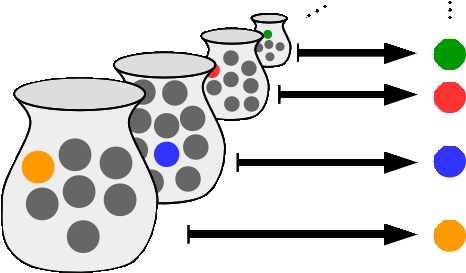
\includegraphics[valign=m,width=7em]{choice-function}}
      ([yshift=-0.5ex]pic cs:end);
  \end{tikzpicture}
  \vspace*{-1.5em}
  \pause

  \hil{Note.} The axiom of choice is \hil{superfluous} for \ldots
  \vspace*{-2em}
  \begin{columns}
    \small
    \begin{column}{0.25\textwidth}
      \begin{enumerate}
        \item[\bignumber{A}] \hil{finite} collections
      \end{enumerate}
    \end{column}
    \begin{column}{0.67\textwidth}
      \begin{enumerate}
        \item[\bignumber{B}] collections of inhabited decidable sets of natural numbers
      \end{enumerate}
    \end{column}
  \end{columns}
\end{frame}}

\newcommand{\Fbox}[1]{{\color{gray!50}\fbox{\color{black}#1}}}
\newcommand{\konfig}[6]{
  \ldots
  \Fbox{\ensuremath{\stackrel{#1}{
\includegraphics[height=0.4em]{player-1}}}}\
  \Fbox{\ensuremath{\stackrel{#2}{
\includegraphics[height=0.4em]{player-2}}}}\
  \Fbox{\ensuremath{\stackrel{#3}{
\includegraphics[height=0.4em]{player-3}}}}\
  \Fbox{\ensuremath{\stackrel{#4}{
\includegraphics[height=0.4em]{player-4}}}}\
  \Fbox{\ensuremath{\stackrel{#5}{
\includegraphics[height=0.4em]{player-5}}}}\
  \Fbox{\ensuremath{\stackrel{#6}{
\includegraphics[height=0.4em]{player-6}}}}
  \ldots}

\begin{frame}{What a choice function can do for us in the riddle}
  \jnote{1-}{
    For the purposes of the slide, two scenarios being ``almost-identical''
    means that they differ at most at finitely many positions.

    As every team member knows the numbers of all the others, every team member
    can identify with certainty the correct set of almost-identical scenarios.
    If they would now each pick an inhabitant of that set independently of each
    other, nothing would be gained. But if they all know a common choice
    function, they can use it to coordinate their guesses without violating
    the rule of no-communication.

    The existence of such a choice function is guaranteed by the axiom of
    choice. Hence, assuming the axiom of choice, there at least \emph{exists} a
    winning strategy for the mathematicians. (Whether they have access to this
    strategy is a different question.)
  }

  \small
  For the collection of \hil{sets of almost-identical scenarios}, a choice function
  could look like this:
  \[
    \small
    \begin{array}{ccc}
      \left\{
        \begin{array}{c}
          \konfig{3}{3}{3}{3}{3}{3} \\
          \konfig{3}{3}{3}{1}{3}{3} \\
          \konfig{3}{3}{3}{1}{1}{3} \\
          \text{(and many more scenarios)}
        \end{array}
      \right\} &\longmapsto&
      \konfig{3}{3}{3}{3}{3}{3} \\
      \\[-1em]
      \left\{
        \begin{array}{c}
          \konfig{1}{2}{1}{2}{1}{2} \\
          \konfig{1}{2}{1}{4}{1}{2} \\
          \konfig{1}{2}{1}{5}{1}{2} \\
          \text{(and many more scenarios)}
        \end{array}
      \right\} &\longmapsto&
      \konfig{1}{2}{1}{2}{1}{2} \\
      \\[-1em]
      \text{(and many more sets)} && \text{(and many more representatives)}
    \end{array}
  \]

  \begin{columns}[c]
    \begin{column}{0.00\textwidth}
      \vspace*{0.5em}
\includegraphics[valign=m,height=1.0em]{lightbulb}
    \end{column}
    \begin{column}{0.9\textwidth}
      If the players use a \hil{common choice function} to make
      their guesses, \\ \hil{only finitely many} will be incorrect.
    \end{column}
  \end{columns}
\end{frame}

\begin{frame}{Consequences of the axiom of choice}
  \jnote{1}{
    To properly assess a proposed axiom for mathematics, we should not only
    philosophically connect with its statement, but also explore the
    consequences it entails. One reason that the axiom of choice is somehow contested is
    that, somehow unusual for a foundational axiom, it entails both consequences which are commonly considered ``bad'' and
    consequences which are considered ``good'' (but which I personally prefare
    to reframe as ``procrastinatory'').

    Among the ``bad'' consequences are the following counterintuitive results:
    \begin{enumerate}
      \item There is a winning strategy for the mathematicians challenged by the evil monster.
      \item There are shapes in the usual three-dimensional space of such weird form that,
      provably so, there is no reasonable way of assigning them a volume (not
      even the extremal values $0$ or~$\infty$ cubic units).
      \item A solid three-dimensional ball can be disassembled into five
      pieces in such a way that these pieces can be reassembled (after
      rotation and translation) to form two disjoint copies of the original
      ball, each of the same size as the original ball.
      \item A certain form of prophecy is possible (see link).
    \end{enumerate}
  }

  \jnote{2-}{
    In many cases, a more detailed analysis enables us to cope with losing the
    consequences usually deemed ``good''. For instance:
    \begin{enumerate}\justifying
      \item While~\textsc{ac} is required to ensure that every field has an
      algebraic closure, the following fact can be established without it:
      Every field has an algebraic closure \emph{in a certain extension of the
      mathematical universe}. This ``sheaf-theoretic substitute'' can serve
      similar purposes as a true algebraic closure existing in the same
      universe.

      \emph{Some results otherwise obtained using the axiom of choice can be
      recovered if we are prepared to travel the toposophic multiverse and pass
      to extensions of the universe.}
      \item While~\textsc{ac} is required for several infrastructural tools,
      concrete results obtained with these tools can often be recovered without
      appealing to~\textsc{ac}. This is ascertained by certain meta theorems
      concerning Gödel's sandbox (introduced below).
    \end{enumerate}
  }

  \centering
  \hil{``Weird'':}
  \medskip
  \begin{columns}
    \begin{column}{0.2\textwidth}
      \centering
      \fixedhref{https://infinityplusonemath.wordpress.com/2017/10/31/non-measurable-sets-that-go-bump-in-the-night/}{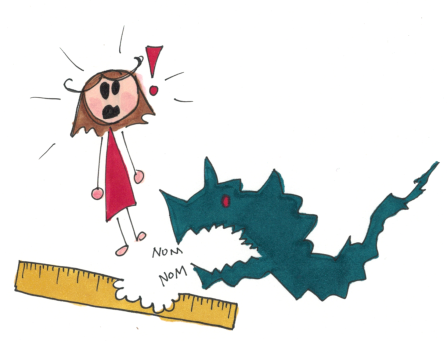
\includegraphics[height=4em]{non-measurable-monster}} \\
      Vitali fractal
    \end{column}
    \begin{column}{0.6\textwidth}
      \centering
      \fixedhref{https://en.wikipedia.org/wiki/Banach\%E2\%80\%93Tarski_paradox}{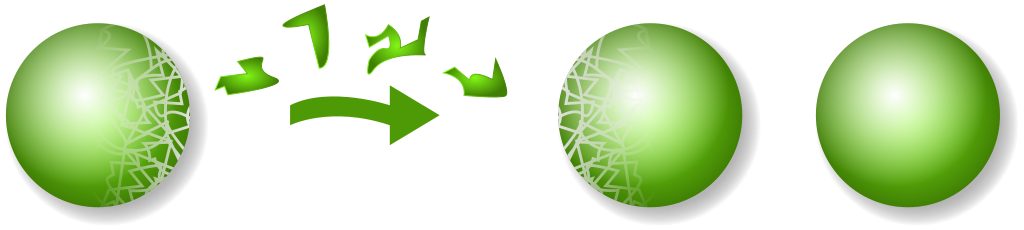
\includegraphics[height=4em]{banach-tarski}}
      Banach--Tarski paradox
    \end{column}
    \begin{column}{0.15\textwidth}
      \centering
      \fixedhref{https://mathoverflow.net/questions/151286/probabilities-in-a-riddle-involving-axiom-of-choice}{
\includegraphics[height=4em]{crystal-ball}}
      Prophecy
    \end{column}
  \end{columns}
  \bigskip
  \bigskip

  \hil{``Good/procrastinatory'':}
  \medskip
  \begin{columns}
    \begin{column}{0.5\textwidth}
      \centering
      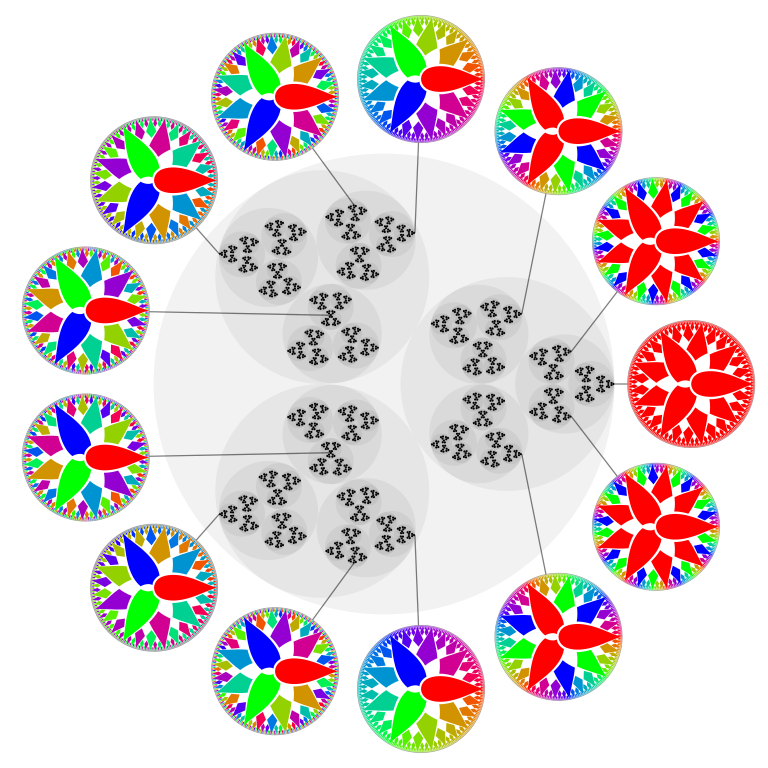
\includegraphics[height=4em]{p-adic} \\
      Every field has an algebraic closure.
    \end{column}
    \begin{column}{0.4\textwidth}
      \centering
      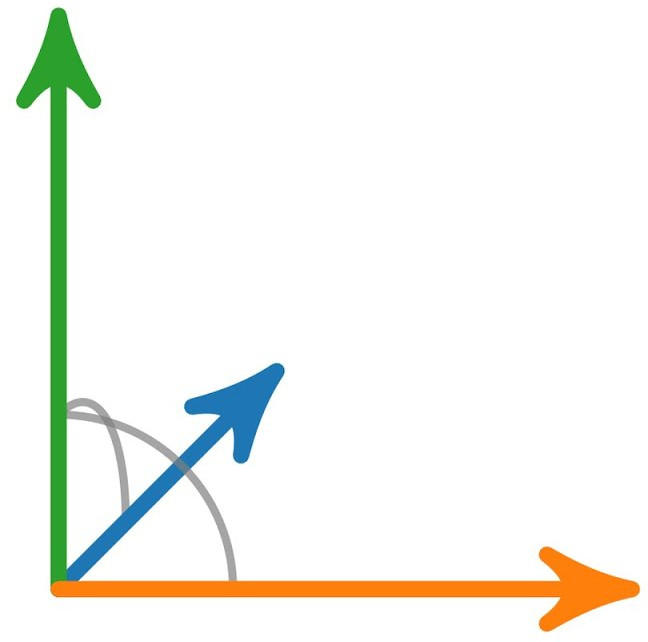
\includegraphics[height=4em]{basis} \\
      Every vector space has a basis.
    \end{column}
  \end{columns}
\end{frame}

\newcommand{\expl}[2]{
  \justifying
  ``$\!\text{\normalnumber{#1}}$'' in the effective topos amounts to: #2
}
\newcommand{\qswitch}[3]{\only<1-#1>{
\includegraphics[height=0.7em]{question-mark}}\only<#2->{#3}}
\newcommand{\ccmark}{\good{\cmark}}
\newcommand{\cxmark}{\bad{\xmark}}
\newcommand{\notnot}{\emph{not~not}\xspace}
\begin{frame}{An alternative universe: the effective topos}
  \jnote{1-}{
    Besides the standard mathematical universe we are introduced to in school,
    there is a host of alternative mathematical universes (models of set
    theory, or, more generally, toposes, or even more generally models of type
    theory). Every such universe has its own stock of mathematical objects like
    numbers, shapes and functions, any none of these universes is too alien---in all
    alternative mathematical universes it holds that $2 + 2 = 4$ and that there
    are infinitely many prime numbers. However, in certain other aspects
    mathematics unfolds differently in those alternative universes.

    In the particular alternative universe known as the \hil{effective topos},
    exactly those statements are true which have a computational witness (by a
    Turing machine). As sketched on the next slide,~\textsc{ac} has no
    such witness---\emph{the effective topos harbors a counterexample to the
    axiom of choice}.

    All mathematical universes support \hil{constructive reasoning}, that is
    reasoning without using the axiom of choice and without using the law of
    excluded middle. Universes in which these axioms do hold are rather
    special. This fact of life (unrelated to philosophical beliefs) is one of
    the main reasons to do without the axiom of choice:

    \begin{quote}
      Appealing to the axiom of choice restricts the scope of our mathematical
      arguments to the few universes supporting that axiom. The axiom of choice,
      and also already the law of excluded middle, precludes computational (and
      geometric) interpretations of the logical connectives.
    \end{quote}

    \href{https://arxiv.org/abs/2204.00948}{Check here for a primer on
    alternative mathematical universes.}
  }

  \centering
  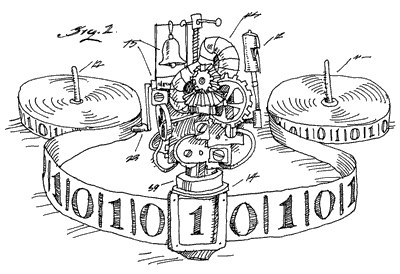
\includegraphics[width=7em]{turing-machine}
  \small

  \begin{tabular}{@{\!\!\!\!\!\!}l@{\,}llp{1.8cm}}
    \toprule
    & statement & in $\mathsf{Std}$ & in $\mathsf{Eff}$ \\
    \midrule
    \normalnumber{1} & Every number is prime or not prime. & \ccmark{}
    (trivially) & \ccmark \\
    \normalnumber{2} & Beyond every number there is a prime. & \ccmark & \ccmark \\
    \normalnumber{3} & Every map $\NN \to \NN$ has a zero or not. & \ccmark{} (trivially) & \cxmark \\
    \normalnumber{4} & Every map $\NN \to \NN$ is computable. & \cxmark &
    \qswitch{4}{5}{\ccmark}\only<1-4>{\,} \visible<5->{(trivially)} \\
    \normalnumber{5} & Every map $\RR \to \RR$ is continuous. & \cxmark &
    \qswitch{5}{6}{\ccmark{} (if MP)} \\
    \normalnumber{6} & Every map $\NN \to \NN$ which does \notnot{} have a zero
    has a zero. & \ccmark{} (trivially) &
    \qswitch{6}{7}{\ccmark{} (if MP)} \\
    %\normalnumber{7} & Countable choice holds. & \ccmark &
    %\qswitch{7}{8}{\ccmark{} (always!)} \\
    %\normalnumber{8} & Heyting arithmetic is categorical. & \cxmark &
    %\qswitch{8}{9}{\ccmark{} (if MP)} \\
    %\normalnumber{9} & A statement holds iff it is realized. & \cxmark &
    %\qswitch{9}{10}{\ccmark} \\
    \bottomrule
  \end{tabular}
  \medskip

  \only<1>{\color{white}There is a machine which determines of any given
  number whether it is prime or not. \\\ \\\ }
  \only<2>{\expl{1}{There is a machine which determines of any given
  number whether it is prime or not. \\\ \\\ }}
  \only<3>{\expl{2}{There is a machine which, given a number~$n$, computes a
  prime larger than~$n$. \\\ \\\ }}
  \only<4>{\expl{3}{There is a machine which, given a machine
  computing a map~$f : \NN \to \NN$, determines whether~$f$ has a
  zero or not. \\\ \\\ }}
  \only<5>{\expl{4}{There is a machine which, given a machine
  computing a map~$f : \NN \to \NN$, outputs a machine
  computing~$f$. \hfill \emph{cat!} \\\ \\\ }}
  \only<7>{\expl{6}{There is a machine which, given a machine
  computing a map~$f : \NN \to \NN$ and given the promise that it is \notnot
  the case that~$f$ has a zero, determines a zero of~$f$. \hfill \emph{unbounded
  search!}}}
  %\only<8>{\expl{7}{\justifying There is a machine which, given a machine
  %computing for every~$x \in \NN$ some~$y \in A$ together with a realizer
  %of~$\varphi(x,y)$, outputs a machine computing a suitable choice
  %function~$\NN \to A$.}}
  %\only<9>{\ \\\ \\\ \\\ }
  \bigskip
  \pause
  \pause
  \pause
  \pause
  \pause
  \pause
  \pause

  \begin{columns}
    \begin{column}{0.00\textwidth}
      \dbend
    \end{column}
    \begin{column}{0.9\textwidth}
      In $\mathsf{Eff}$, there is \hil{no choice function} for the collection of \\
      \hil{sets of behaviourally identical programs}.
    \end{column}
  \end{columns}
\end{frame}

\begin{frame}{A counterexample to the axiom of choice}
  A \hil{choice function} for the collection of \hil{sets of behaviourally
  identical programs} could look like this:
  \[
    \small
    \begin{array}{lll}
      \left\{
        \begin{array}{l}
          \textsf{while True: pass} \\
          \textsf{while 2 == 1 + 1: pass} \\
          \textsf{s = "a"; while len(s) > 0: s = s + "a"} \\
          \vdots
        \end{array}
      \right\} &\longmapsto&
      \textsf{while True: pass} \\
      \\[-0.5em]
      \left\{
        \begin{array}{l}
          \textsf{print(2+2)} \\
          \textsf{print(4)} \\
          \textsf{print(len("37c3"))} \\
          \vdots
        \end{array}
      \right\} &\longmapsto&
      \textsf{print(4)} \\
      \\[-0.5em]
      \vdots && \vdots
    \end{array}
  \]

  With such a choice function~\textsf{c}, a \hil{halting oracle} could be built: \\
  A program~$p$ loops if and only if~$\textsf{c}(p) = \textsf{c}(\textsf{"while True: pass"})$.
\end{frame}

\newcommand{\Fboxs}[1]{\Fbox{\begin{minipage}[c][2em]{2em}\centering\ensuremath{#1}\end{minipage}}}
\begin{frame}{A varied perspective on the axiom of choice}
  \jnote{2-3}{
    Glossary of foundational systems mentioned on the slide:
    \begin{itemize}
      \item {\justify \textsc{zfc}, Zermelo--Fraenkel set theory with the axiom of choice,
      is often quoted as the standard foundational system for mathematics
      commonly accepted by logicians. (This claim should be taken with a grain
      of salt: While it is true that most of contemporary mathematics can be
      formalized in~\textsc{zfc}, there are important exceptions (such as large
      structures in category theory), and other systems (such as certain
      flavors of type theory) are also up to that task. Most mathematicians
      work informally, on a higher level, polymorphically in the foundation,
      and couldn't recite the~\textsc{zfc} axioms when asked.)\par}
      \item \textsc{zf} is the variant of~\textsc{zfc} without~\textsc{ac}.
      \item \textsc{pra} is a certain base theory so weak that it is contested
      just by ultrafinitists and hence often used as a super-safe basis for
      metamathematical pursuits.
    \end{itemize}
    \href{https://iblech.gitlab.io/bb/multiverse.html}{Check here for a recap
    why these systems were put into place and how they are riddled by
    fundamental incompleteness.}
  }

  \jnote{4}{
    Much more severe than the axiom of choice is the \hil{powerset axiom},
    commonly adopted but enabling \hil{impredicative reasoning}.
    
\includegraphics[height=0.8em]{scream}

    Provably so, a sandbox for emulating the powerset axiom in case it is not
    assumed on the meta level is \hil{impossible}: Unlike \textsc{ac} (or the
    also-debated law of excluded middle, which incidentally is implied by
    \textsc{ac}), the powerset axiom vastly increases proof-theoretic strength.

    The strength of predicative set theories can be
    \href{https://en.wikipedia.org/wiki/Bachmann\%E2\%80\%93Howard_ordinal}{looked up on
    Wikipedia}, whereas precisely calibrating the strength of impredicative
    formal systems such as \textsc{zf} is currently well out of reach.
  }

  \jnote{5}{
    Want to hone your \textsc{ac} skills? Here is a harder variant of the
    riddle of the beginning (communicated to me via Christian Sattler by David
    Wärn):

    An evil monster prepares a secret chamber containing infinitely many opaque
    boxes. The boxes are numbered by the naturals and each box contains a real
    number of the monster's choosing:
    \[
      \stackrel{\Fboxs{\pi}}{0}\
      \stackrel{\Fboxs{17}}{1}\
      \stackrel{\Fboxs{-\tfrac{1}{3}}}{2}\
      \stackrel{\Fboxs{\sqrt{2}}}{3}\
      \ldots
    \]

    One by one, the evil monster privately guides the members of a team of 100
    mathematicians into the chamber, with the other members waiting outside.
    While in the chamber, each mathematician may open as many boxes as they
    wish, even infinitely many, inspecting their contents. They may base their
    decision as to which boxes to open on the contents they have seen so far.
    The only requirement is that they keep one box of their choosing untouched:
    The monster will ask them for a guess regarding the contents of that box.

    The mathematicians win as a team if and only if at most one of them guesses
    incorrectly. As usual, communication among the team is allowed only
    beforehand. Between successive visits to the chamber, the chamber is reset
    to its original state (so all the opened boxes are closed again).
  }

  \begin{enumerate}
    \item There is an alternate opposing axiom, the \hil{axiom of determinacy}
    (\textsc{ad}): \\
    ``Every instance of the \hil{infinite sequence game} is \hil{determined}.''

    {\small\justifying
    Just as with \textsc{ac}, the finitary version of \textsc{ad}
    follows from uncontested basic axioms.
    \emph{\textsc{ac} and \textsc{ad} constitute different
    extrapolations from the finite to the general domain.}\par}
    \bigskip
    \pause

    \item\justifying Introducing the axiom of choice does \hil{not} yield \hil{new} inconsistencies
    (if~\textsc{zfc} is inconsistent, then~\textsc{zf} is as well---provably so
    in weak metatheories such as~\textsc{pra}).

    {\small\emph{Hence worries about inconsistency arising from the axiom of choice are
    unfounded.}}
    \bigskip
    \pause

    \item Even if \textsc{ac} fails, it always holds in~$L$, \hil{Gödel's sandbox}.
    Amazingly, \textsf{Std}'s and~$L$'s~$\NN$ coincide, hence \textsf{Std} and
    $L$ share the same \hil{arithmetic truths} and hence
    from every proof of such a truth, any appeals to \textsc{ac}
    can be \hil{mechanically eliminated}.

    {\small\emph{Thus \textsc{ac}
    can be regarded as \hil{convenient fiction}, similar to how negative
    numbers are useful but we could always make do with tracking assets and
    debts separately. \textsc{ac} is required for certain general infrastructural
    tools, but superfluous for arithmetic consequences of such tools.}\par}
    \bigskip
    \pause
  \end{enumerate}
\end{frame}

\addtocounter{framenumber}{-1}
\begin{frame}[plain]
  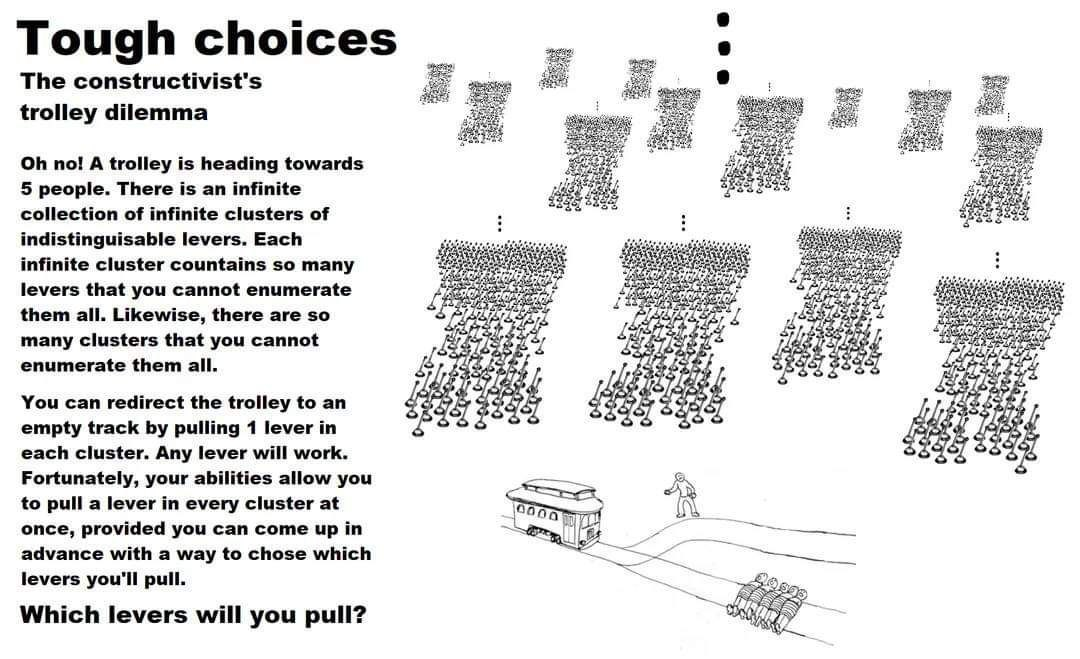
\includegraphics[width=\textwidth]{tough-choices}
\end{frame}

\end{document}
